\documentclass{article}
\usepackage[utf8]{inputenc}
\usepackage[spanish]{babel}
\usepackage{listings}
\usepackage{graphicx}
\graphicspath{ {images/} }
\usepackage{cite}

\begin{document}

\begin{titlepage}
    \begin{center}
        \vspace*{1cm}
            
        \Huge
        \textbf{Parcial 1}
            
        \vspace{0.5cm}
        \LARGE
        Informática II
            
        \vspace{2.5cm}
            
        \textbf{Alejandra Calle Vasquez\\
                Jesús David Mercado Machado \\
                Juan Sebastian Garavito Gallo}
            
        \vfill
            
        \vspace{0.7cm}
            
        \Large
        Despartamento de Ingeniería Electrónica y Telecomunicaciones\\
        Universidad de Antioquia\\
        Medellín\\
        Abril de 2021
            
    \end{center}
\end{titlepage}

\tableofcontents
\newpage
\section{Analisis del problema}\label{intro}
\textbf{Organización de los leds: }
Para la optimización de la conexión y organización de los leds usamos 8 integrados 74HC595 los cuales nos permiten formar un sistema de ubicación de cada bombillo, a cada uno de estos integrados le asignamos 8 leds; que sería lo máximo que podríamos controlar por cada uno de ellos, de este modo formariamos la matriz 8x8 que se es requerida para realizar el ejercicio. Esta manera de conexión de los leds nos pareció optima por que solo conlleva al uso de tres pines.

\section{Circuito inicial en Tinkercad} \label{imagenes}

\begin{figure}[h]
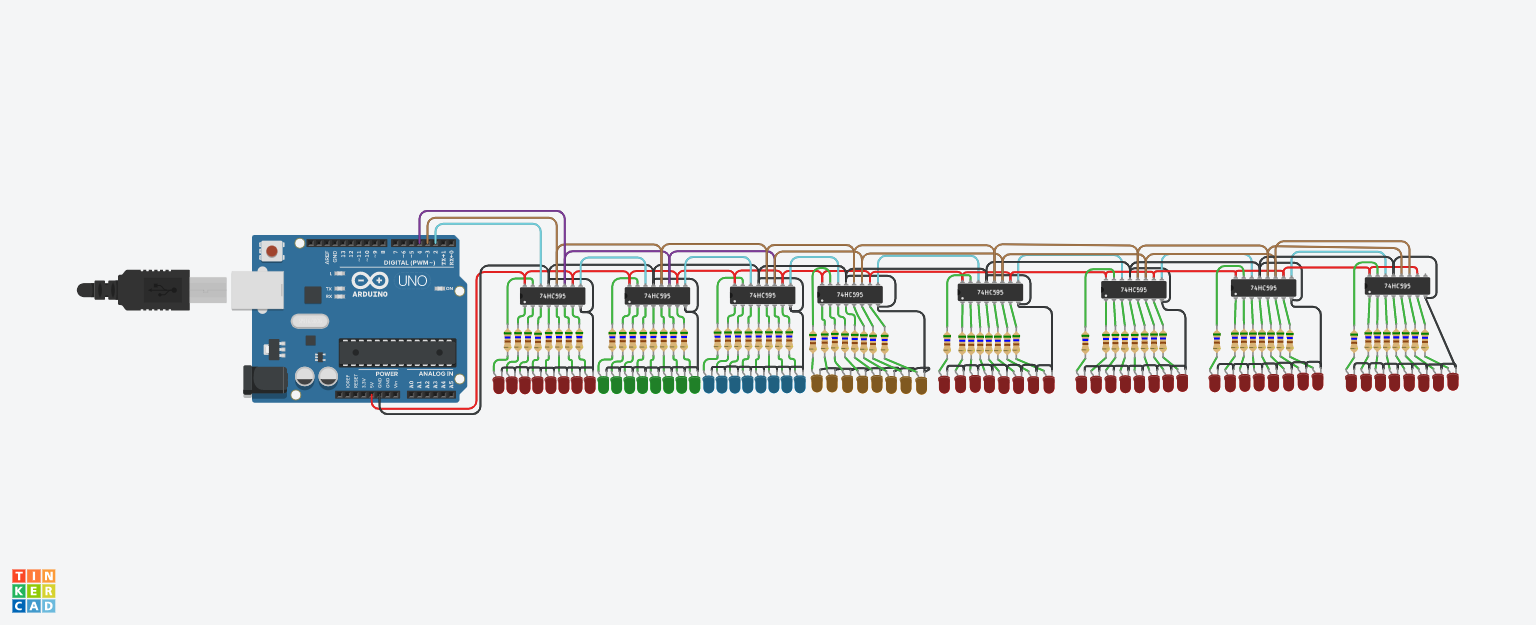
\includegraphics[width=15cm]{PARCIAL INFO 2.png}
\centering
\caption{Primeras conexiones}
\label{fig:PARCIAL INFO 2}
\end{figure}

\vspace*{2cm}

\textbf{Organización matricial de los leds: }
En este caso organizamos nuestros leds de modo que se pueda ver el tablero en forma de matriz y usamos unos patrones establecidos para corroborar su funcionamiento. 

\newpage

\subsection{}
Para representar estos codigos predeterminados usaremos entradas de 1 y 0 para representar los patrones con las siguientes clasificaciones
\textbf{1=Endendido}
\textbf{0=Apagado}

\begin{figure}[h]
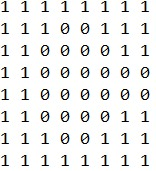
\includegraphics[width=2cm]{imagenC.jpeg}
\caption{Simulación del tablero, signo C}
\label{fig:imagenC}
\end{figure}

\begin{figure}[h]
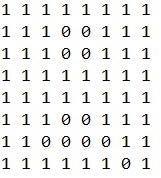
\includegraphics[width=2cm]{imagenB.jpeg}
\caption{Simulación del tablero, signo B}
\label{fig:imagenB}
\end{figure}





\end{document}
